%!TEX program = lualatex
\documentclass[11pt,class=book]{standalone}
%!TEX root = ./main.tex
%!TEX encoding = UTF-8 Unicode

% Pro­gram­ming fa­cil­i­ties
\usepackage{etoolbox}
\usepackage{ifxetex}
\usepackage{ifluatex}

% Encoding
\usepackage[T1]{fontenc}
\ifboolexpr{bool{xetex} or bool{luatex}}{%
	\usepackage{fontspec}
}{%
	\usepackage[utf8]{inputenc}
}

% General purpose
\usepackage{tcolorbox}

% Mathematics
\usepackage{amsmath}
\usepackage{amssymb}
\usepackage{mathrsfs}
\usepackage{amsthm}
\usepackage{dsfont}
\usepackage{braket}
\usepackage{stmaryrd}

% Tables
\usepackage{array}
\usepackage{tabularx}
\usepackage{longtable}
\usepackage{tabu}
\usepackage{booktabs}
\usepackage{multirow}
\usepackage{makecell}
\usepackage{blkarray}

% Figures
\usepackage[mode=tex]{standalone}
\usepackage{import}
\usepackage{float}
\usepackage[justification=centering]{caption}

% PGF-TikZ
\usepackage{pgf}
\usepackage{pgfplots}
\pgfplotsset{compat=1.16}
\usepackage{tikz}
\usepackage{tikzpeople}
\usepackage{pgf-umlsd}
\usepackage{pgfgantt}

%!TEX encoding = UTF-8 Unicode

\usetikzlibrary{shapes}
\usetikzlibrary{arrows.meta}
\usetikzlibrary{calc}

\definecolor{bg_color}{RGB}{250,250,229}

\colorlet{color1}{cyan!50}
\colorlet{color2}{red!30!green!40}
\colorlet{color3}{orange!50}
\colorlet{color4}{violet!60!blue!55}

\definecolor{Cblue}{RGB}{38,75,150}
\definecolor{Cgreen}{RGB}{39,179,118}
\definecolor{Cdarkgreen}{RGB}{0,111,60}
\definecolor{Corange}{RGB}{249,167,62}
\definecolor{Cred}{RGB}{191,33,47}

\newganttlinktype{bartobardown}{
	\ganttsetstartanchor{south east}
	\ganttsetendanchor{north west}
	\draw [/pgfgantt/link] (\xLeft, \yUpper) -- (\xRight, \yLower);
}
\newganttlinktype{bartobarup}{
	\ganttsetstartanchor{north east}
	\ganttsetendanchor{south west}
	\draw [/pgfgantt/link] (\xLeft, \yUpper) -- (\xRight, \yLower);
}
\newganttlinktype{milestonetobardown}{
	\ganttsetstartanchor{south}
	\ganttsetendanchor{north west}
	\draw [/pgfgantt/link] (\xLeft, \yUpper) -- (\xRight, \yLower);
}
\newganttlinktype{bartomilestonedown}{
	\ganttsetstartanchor{south east}
	\ganttsetendanchor{north}
	\draw [/pgfgantt/link] (\xLeft, \yUpper) -- (\xRight, \yLower);
}


\begin{document}
	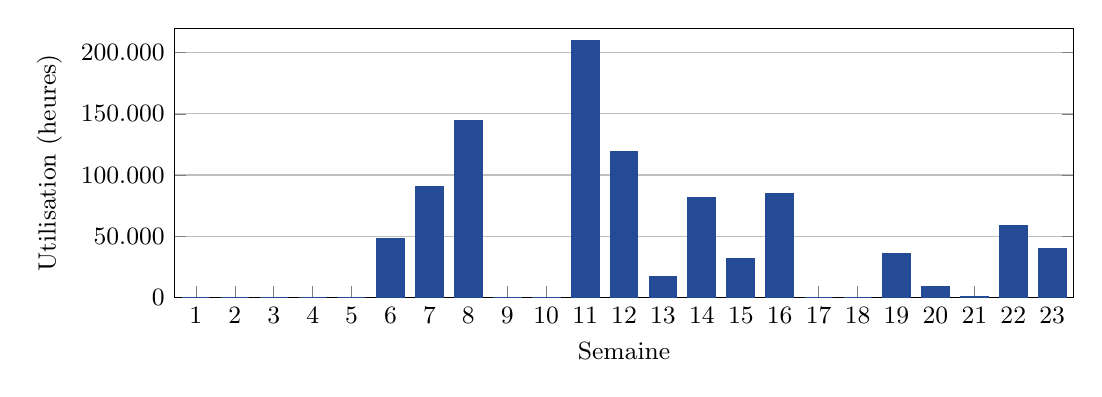
\begin{tikzpicture}[
		x=1pt,
		y=1pt,
		%/utils/exec={\sffamily},
		font=\fontsize{9pt}{9.5pt}\selectfont,
		%>={Triangle[length=4,width=3]},
		%decoration={snake,segment length=5,amplitude=0.7},
	]
		\begin{axis}[
			%ybar,
			width=13cm,
			height=5cm,
			%xmin=0, xmax=22,
			ymin=0, ymax=220000,
			enlarge x limits=0.025,
			%bar width=1,
			%axis lines=none,
			%xtick=\empty,
			%ytick=\empty,
			ymajorgrids=true,
			%yminorgrids=true,
			xtick distance=1,
			xtick=data,
			%tick label style={font=\tiny},
			xtick pos=left,
			xlabel={Semaine},
			ylabel={Utilisation (heures)},
			%nodes near coords,
			%symbolic x coords={1,2,3,4,5,6,7,8,9,10,11,12,13,14,15,16,17,18,19,20,21,22,23},
			y tick label style={
				/pgf/number format/.cd,
				scaled y ticks = false,
				set thousands separator={.},
				fixed
			},
		]
		\addplot[
			ybar,
			Cblue,
			fill=Cblue
		] coordinates {
			(1, 0)
			(2, 0)
			(3, 0)
			(4, 0)
			(5, 0)
			(6, 47789)
			(7, 90261)
			(8, 144885)
			(9, 274)
			(10, 63)
			(11, 209978)
			(12, 119145)
			(13, 16704)
			(14, 81971)
			(15, 31917)
			(16, 84555)
			(17, 0)
			(18, 0)
			(19, 35992)
			(20, 8639)
			(21, 658)
			(22, 58668)
			(23, 39705)
		};
		\end{axis}
	\end{tikzpicture}
\end{document}
